%Template file for Scientific Computation project 1 discussion and figures
\documentclass{article}
\usepackage[a4paper, margin=1in]{geometry}
\title{Scientific Computation Project 1}
\usepackage{minted}
\usepackage{amsmath}
\usepackage{amssymb}
\newcommand{\trm}{\textrm}
\newcommand{\pa}{\partial}
\author{\emph{02046683}}

\usepackage{graphicx}

\begin{document}

\maketitle

%---------------- Part 1  -------------------
\hrule
\hrule

\subsection*{Part 1}

\subsubsection*{1(a)}
\textbf{Method 1} is a simple linear search, where it iterates through the list \( L \) and checks if \( x \) is present.  
\textbf{Method 2} sorts the list of IDs using merge sort first if the list is not sorted, then performs a binary search to find the element.

\subsubsection*{1(b)}
\textbf{Method 1}: \( O(mn) \) since it’s a simple linear search with \( m \) multiple times, using the results from lecture notes. \\
\textbf{Method 2}: For the worst case, we need to sort the list with complexity \( O(n \log_2 n) \), then apply binary search with complexity \( O(m \log_2 n) \).
Hence, the total complexity is \( O((m + n) \log_2 n) \).


\subsubsection*{2.}
%Place your discussion for question 2 here
 To compare the performance of Method 1 and Method 2, we can fix either the size of \( m \) or \( n \) and compare \( O(mn) \) with \( O((m + n) \log_2 n) \).  
Firstly, we fix the value of \( n \) (using \( n = 100 \) and \( n = 10000 \) in the code), and results are shown in Figure 1 and Figure 2.  
The results show that for small \( m \) ( \( m < 150 \) in the graphs), Method 2 is a little bit slower than Method 1. This can be seen by the mathematical comparison of \( O(mn) \) and \( O((m + n) \log_2 n) \), or by the consideration of the cost of the merge sort in Method 2.  
As the size of \( m \) increases, Method 1 takes much longer time than Method 2 as shown in the graphs. This is because \( O(mn) \) is much bigger than \( O((m + n) \log_2 n) \) if we fix the value of \( n \) for large \( m \). Hence, the results shown in the graphs agree with our theoretical results.

Now, we fix the value of \( m \) (using \( m = 10 \) and \( m = 1000 \) in the code), and the results are shown in Figure 3 and Figure 4.  
For \( m = 10 \) (i.e., \( m \) is small), the results show that there is not much difference between Method 1 and Method 2 as expected for small \( n \).  
As the size of \( n \) increases, Method 2 becomes much slower than Method 1 as shown in the graph, since \( O((m + n) \log_2 n) \) is much bigger than \( O(mn) \) in this case.  
For \( m = 1000 \) (i.e., \( m \) is large), as \( n \) increases, Method 2 is much faster than Method 1, as expected from the comparison of \( O(mn) \) and \( O((m + n) \log_2 n) \).  
Hence, the results shown in the graphs also agree with our theoretical results.

\begin{figure}[h!]
\centering
%Uncomment line below to display figure saved as fig1.png
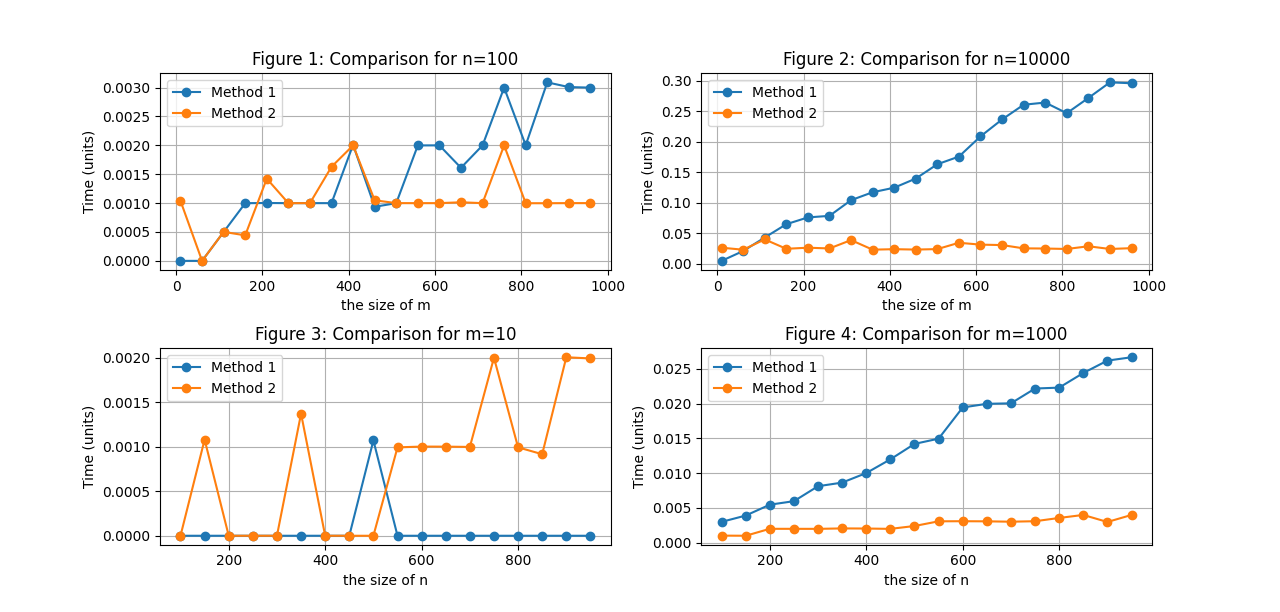
\includegraphics[width=1.1\textwidth]{Figure_1.png}

\caption{The top two figures fix the size of n and vary different values of m. The bottom two figures fix the size of m and vary different values of n. }
\label{fig1}
\end{figure}

%Add additional figure if needed

%---------------- End Part 1 -------------------

\vspace{0.25in}

%---------------- Part 2  -------------------
\subsection*{Part 2}

\subsubsection*{2.}

\textbf{Code Description:}

The function achieves this by:
\begin{enumerate}
    \item For each pair in L, convert the first pattern in L to a numerical form (base-9) for hashing. For example, if one pair in L is ['abc', 'def'], then we only convert 'abc' in base9. 
    \item Using a rolling hash technique to compare the hash value of subsequences of $A_1$ with the hash value of first pattern for each pair in L.
    \item If there is a match, compare the first pattern within $A_1$ and the corresponding second pattern within $A_2$.
    \item If they are all matched, then we add the location to the list $F$.
\end{enumerate} \\

\textbf{Time Complexity:}

The time complexity of the \texttt{part2} function is approximately $ O(m \times l \times ( n-m+1 )) $, where:
\begin{itemize}
    \item \( m \) is the length of the pattern in L.
    \item \( n \) is the length of the amino acid sequences $A_1$ and $A_2$.
    \item \( l \) is the number of patterns in list L.
\end{itemize}

The primary components contributing to this complexity come from the updation of the rolling hash:
\begin{itemize}
    \item Going through all the sublists of $A_1$ gives the $O(n-m+1)$ complexity.
    \item Checking if the sublist of $A_1$ matches with the patterns in L gives the $O(l)$ complexity.
    \item Checking if the patterns of L both match with $A_1$ and $A_2$ gives the $O(m)$ complexity.
\end{itemize}


\textbf{Why This Code is Efficient:}

The \texttt{part2} function is efficient due to the use of a rolling hash algorithm, which allows for subsequence matching without recomputing hashes from scratch each time. This minimizes unnecessary recomputation and is faster than a direct comparison approach, especially as the input size grows. Also, we only compare the first pattern in L with $A_1$, which reduces the computational cost.


%Place your discussion for question 2 here}
%---------------- End Part 2 -------------------


\hrule
\hrule



%---------------- End document -------------------


\end{document}
